\documentclass[UTF8,a4paper,10pt]{ctexart}
\usepackage[margin=2.5cm]{geometry}
\usepackage{graphicx}
\usepackage{caption}
\usepackage{hyperref}
\setlength{\parindent}{0pt}
\pagestyle{plain}
\begin{document}
{\large 圆柱中部径向模型与控制体}\par\medskip
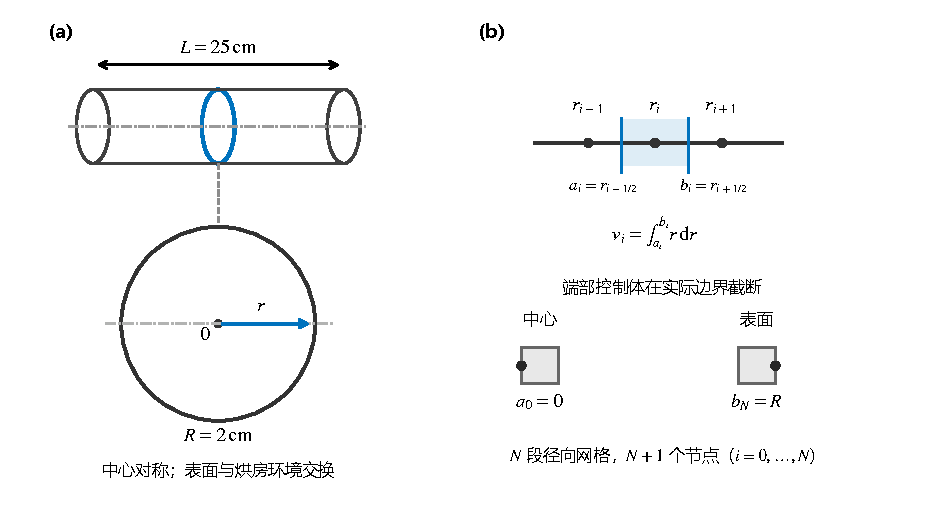
\includegraphics[width=15.8cm]{fig01_radial_model.pdf}\par\smallskip
圆柱及网格均为示意。控制体按径向位置截取圆环，中心与表面控制体分别截断于0与R；图中少量节点不代表正式网格数。
\par\bigskip
\newpage
{\large 烘房环境观测与分段线性重建}\par\medskip
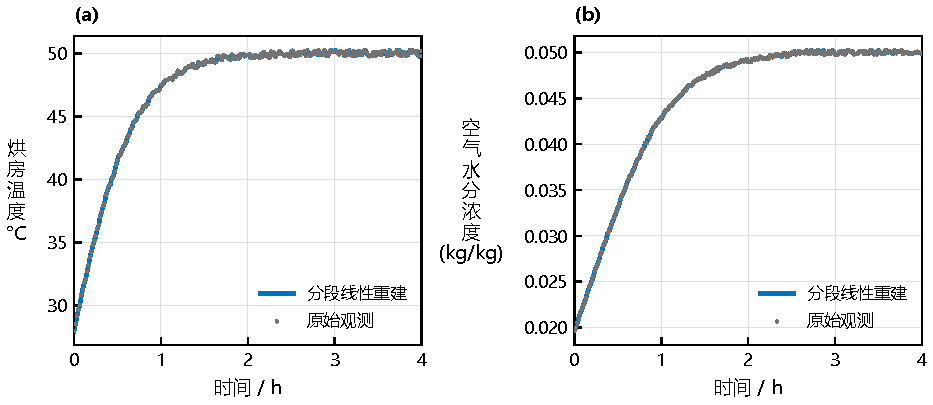
\includegraphics[width=15.8cm]{fig02_environment.pdf}\par\smallskip
两幅图分别表示附件1的温度与空气水分浓度。灰点为241个原始观测，蓝线为分段线性重建。图示0—4 h；Q1仅使用前0.5 h，Q2结果展示前三小时。
\par\bigskip
\newpage
{\large Q1预热阶段温度与含水率的径向响应}\par\medskip
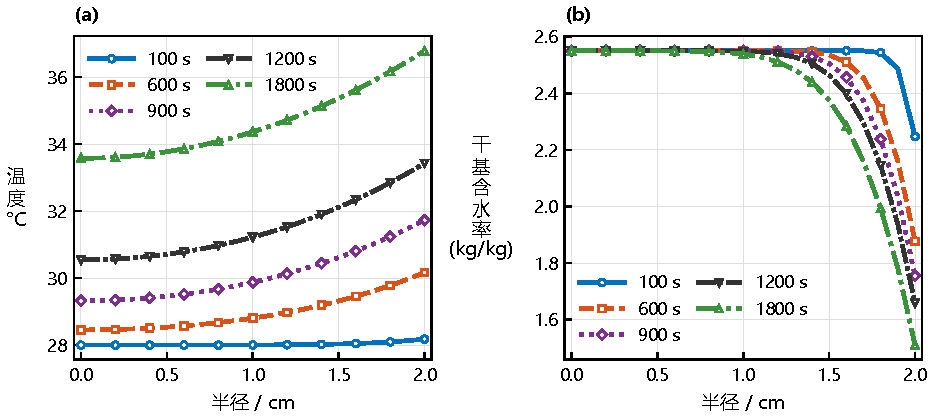
\includegraphics[width=15.8cm]{fig03_q1_profiles.pdf}\par\smallskip
分别绘制100、600、900、1200、1800 s时的温度和干基含水率，均为题目规定的表格时刻。900、1200 s的剖面补充中间阶段的径向变化。每条曲线连接21个规定半径的未舍入计算值，稀疏标记用于识别曲线，未额外拟合。
\par\bigskip
\newpage
{\large Q2前三小时温度与含水率的时空分布}\par\medskip
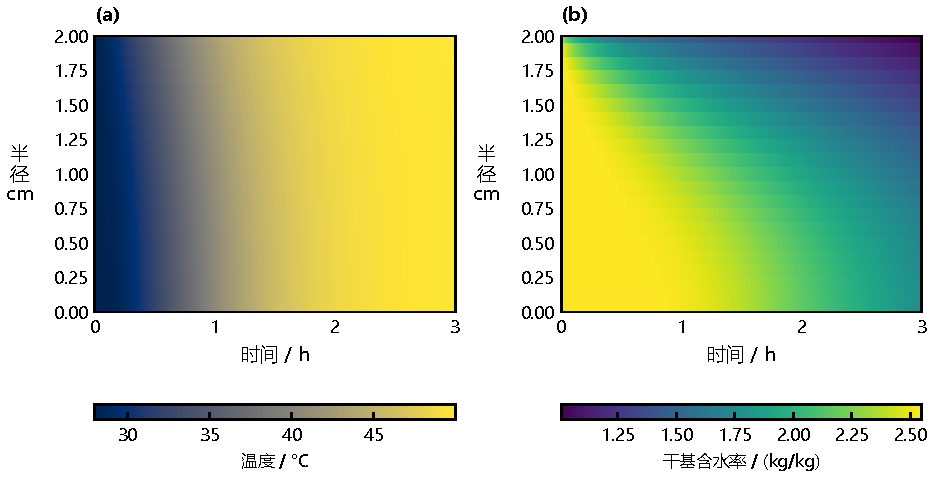
\includegraphics[width=15.8cm]{fig04_q2_fields.pdf}\par\smallskip
横轴为时间，纵轴为实际半径，色标分别表示温度与干基含水率。色场取前三小时逐秒保存的21个规定半径值，采用邻近色块显示；它不表示全部细网格节点的逐秒快照。
\par\bigskip
\newpage
{\large Q3完整干燥过程与全域达标判定}\par\medskip
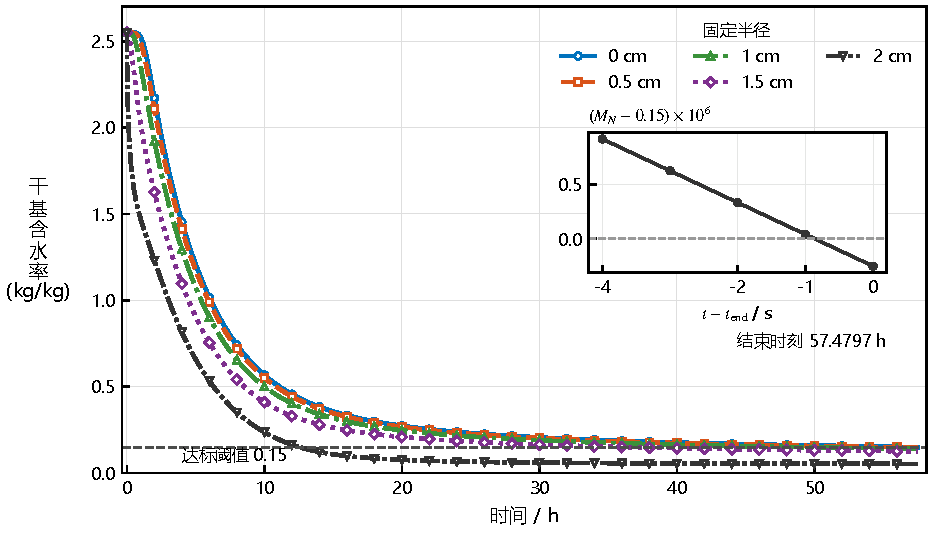
\includegraphics[width=15.8cm]{fig05_q3_drying.pdf}\par\smallskip
主图为五个固定半径的干基含水率历程。小图的M\_N为全10241节点的最大含水率，206926 s尚未严格低于0.15，206927 s首次达标。微小差值只解释数值终点判据，不代表实际干燥时长具有秒级准确度。
\par\bigskip
\newpage
{\large Q4外半径观测与收缩坐标对应}\par\medskip
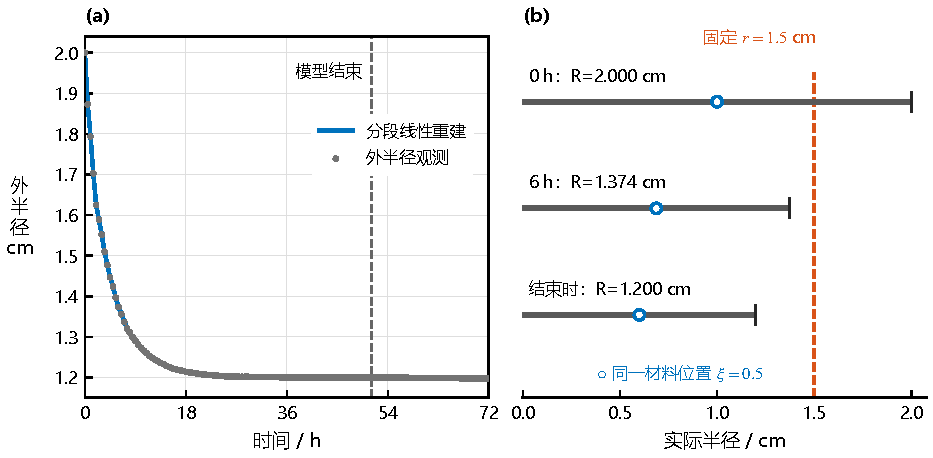
\includegraphics[width=15.8cm]{fig06_q4_geometry.pdf}\par\smallskip
左图展示附件2的0—72 h外半径观测，虚线标出当前模型结束时刻。右图按均匀径向缩放假设绘制r=R(t)$\xi$：同一$\xi$的位置随半径移动，固定r=1.5 cm在6 h时已位于材料外。三行仅排列时刻，内部位置不是实测数据。
\par\bigskip
\newpage
{\large Q4收缩条件下的含水率演变}\par\medskip
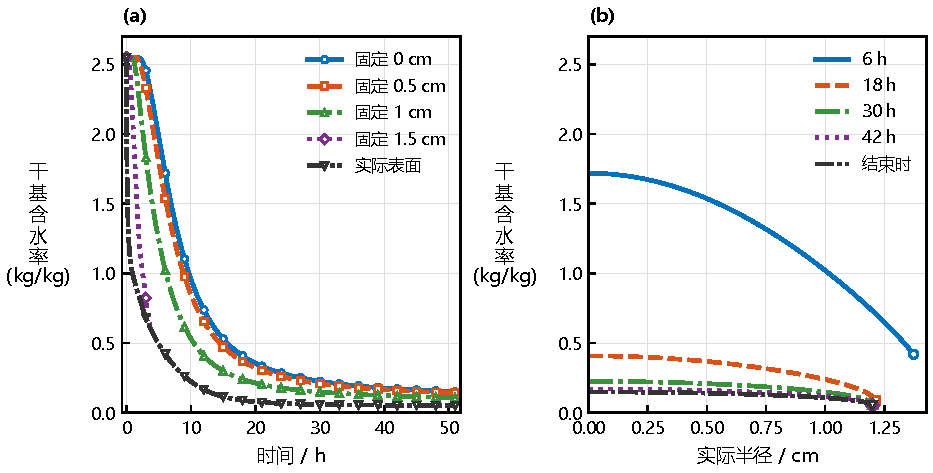
\includegraphics[width=15.8cm]{fig07_q4_profiles.pdf}\par\smallskip
左图采用固定物理位置和实际移动表面的含水率；固定位置移出材料后断线。右图为6、18、30、42 h及结束时的完整细网格剖面，横坐标是实际半径，各曲线端点为当时表面R(t)。
\par\bigskip
\newpage
{\large Q1网格加密的数值一致性}\par\medskip
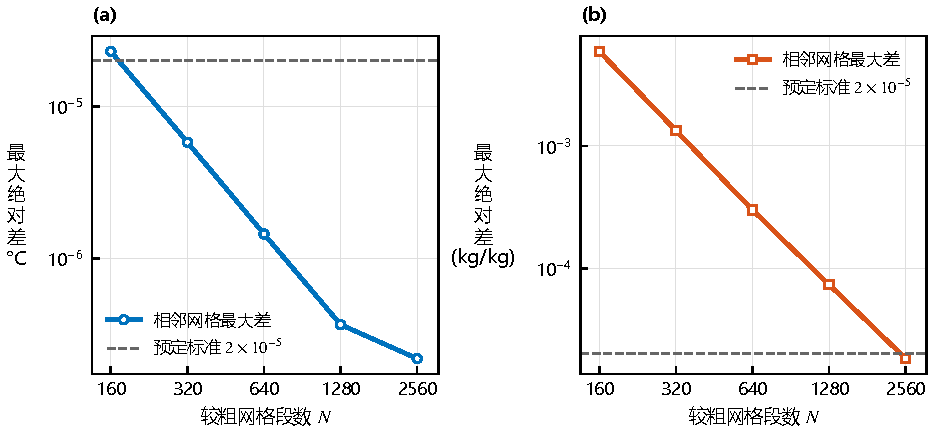
\includegraphics[width=15.8cm]{fig08_grid_convergence.pdf}\par\smallskip
比较N与2N网格在全部1800×21个规定输出点上的最大绝对差。温度和含水率分别显示，虚线为已有预定检验标准。相邻网格差用于评价数值一致性，不是连续解误差的严格上界；本图只对应Q1。
\par\bigskip
\end{document}
